\chapter{Methodology}
\label{methodology}
\iffalse
\begin{itemize}
    \item Requirement validation as base methodology
    \item Test environment (Discussion Mininet vs Distrinet vs our solution)
    \item Protection goals (including metrics like bandwidth and latency)
    \begin{itemize}
        \item Questions that can be validated in chapter “Validation” => Protection goal list
    \end{itemize}
    \item Attackers
    \item Deployments
    \begin{itemize}
        \item Full local deployment
        \item Minimal distributed deployment (2 Hosts, 1 real-world SDN Switch)
    \end{itemize}
\end{itemize}
\fi
\cgn{Is it more logical to move this Methodology after Implementation chapter and before Validation one? Naturally, after discussing the related work and discussing their limitation, one would expect to see the proposed solution (with Design and Implementation).}
\cfw{This chapter is basically split in two parts: Everything until 4.4 covers content that is needed for design and implementation. 4.5 to 4.7 then cover our validation methods. I thus see this chapter as more of a chronological order on how the solution was created and evaluated, before actually performing these actions. The role of the chapter is thus more directed at "what did we do after our research" for me rather than what is immediatly up next in the thesis. Maybe we can discuss this tomorrow in our meeting. It would sure be possible to move 4.5 to 4.7 to the beginning of chapter 7 without many issues.}
To be able to accurately design, implement and validate our solution we will need to specify our methodology first. To achieve our goal we will use requirement validation. Initially we defined our requirements as stated in section \ref{related_work_requirements}.

In this chapter we will thus choose an accurate environment for our experiments, define a network model, our protection goals and attackers, before finally stating the scenarios we wish to validate and our measurements we wish to obtain on them. We will then state all experiments we will perform that will subsequently be evaluated in the validation chapter (see chapter \ref{validation}).

\section{Test environment}
As a test environment we want to use a network emulator to be able to easily bootstrap our solution. For this, multiple emulators are available, including mininet \cite{mininet}, distrinet \cite{distrinet1, distrinet2}, maxinet \cite{maxinet}, ComNetsEmu \cite{comnetsemu} or our own testbed solution \cite{owntb}.

\paragraph{Mininet and ComNetsEmu} emulate network topologies on a single machine, but do not scale to multiple machines. As we want to test in a distributed setting, they are sadly out of the equation.

\paragraph{Distrinet and maxinet} would both allow us to scale mininet topologies to multiple machines. As we want to be able to deploy our topologies to real-world devices in the future though and integrate real-world hardware (requirement R3), we would need to invest additional effort in deploying to real-world hardware in the future when using them.

\paragraph{Our own testbed solution} mitigates these issues by supporting multiple modes of deployment including support for real-world hardware that can easily be extended.

\paragraph{} We will thus opt to use our own hybrid testbed to evaluate our solution.

\section{Network model}
In the context of our networks, we will establish two different kinds of networks.

\begin{figure}[h]
  \centering
  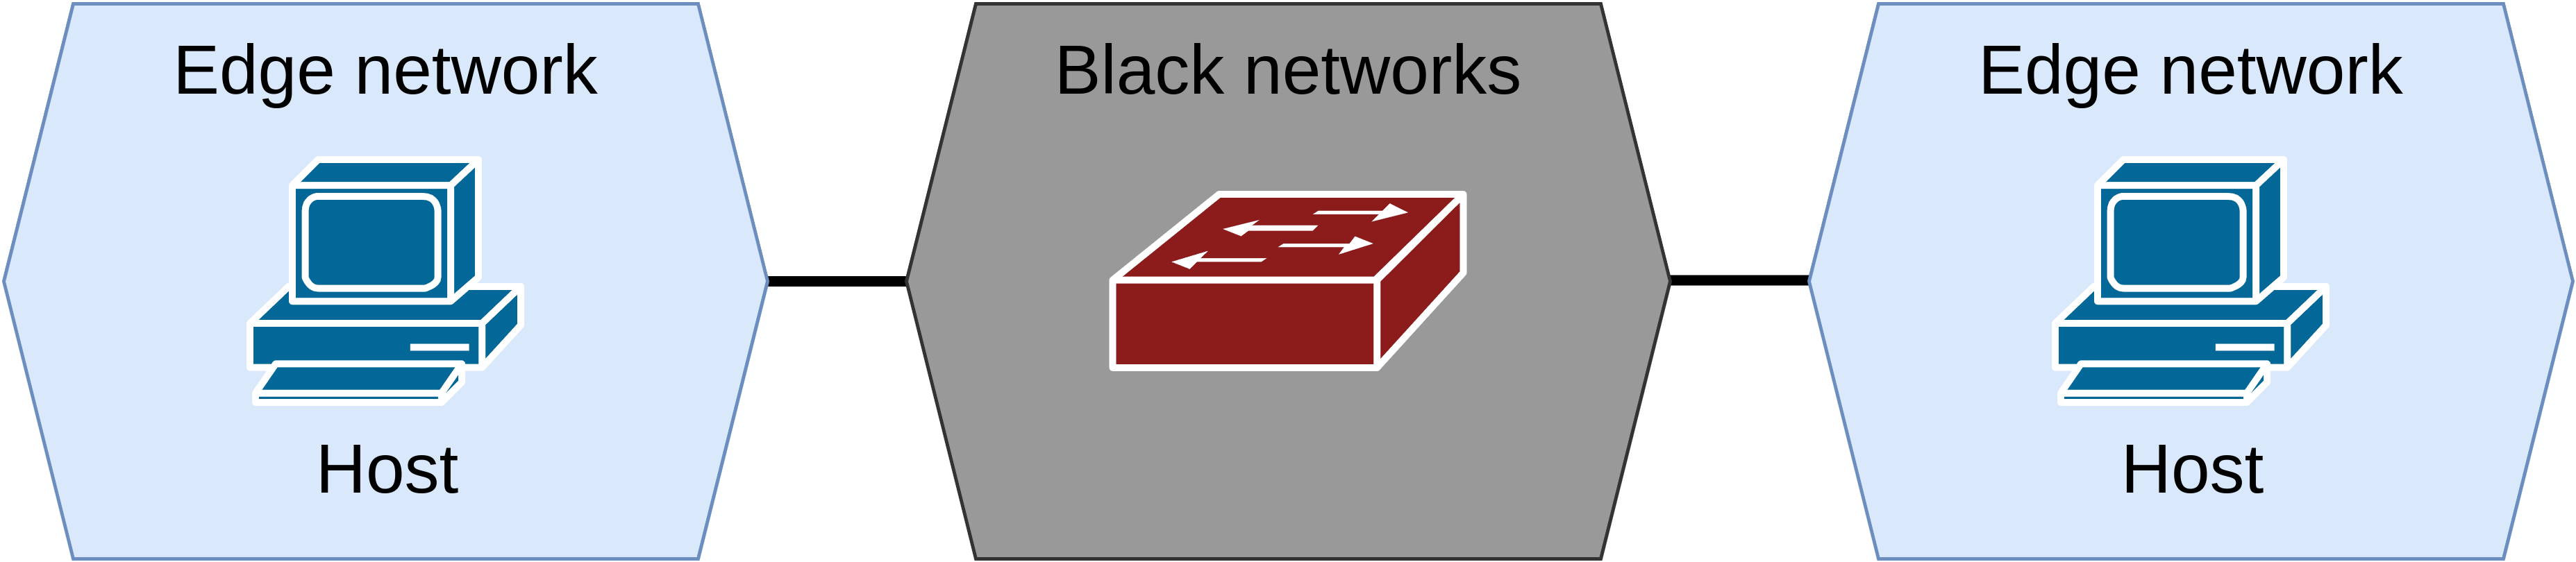
\includegraphics[width=\textwidth]{images/chapter_4/network_model.png}
  \caption[Network model]{Our network model showing the separation of trusted edge networks and semi-trusted black networks. While edge networks are the source and target of our network slice traffic, black networks act as transit networks. There can be multiple black networks between our edge networks, but for simplicity reasons only one of them is indicated in the figure.}
  \label{fig:network_model}
\end{figure}

\paragraph{Edge networks}
are the origin and target of one specific network slice. Each edge network is partially trusted by us, because we or another trusted party operate the core infrastructure. We only expect threats from adversaries outside of our switches or slicing architecture following a zero trust approach, for example as a host established within our edge network.
\paragraph{Black networks}
lie between the edge networks and are operating under a service level agreement (SLA). There may be any number of black networks between two edges, including none. A black network acts as a transit network to us and is semi-trusted because the infrastructure is not operated by us. We do trust that the black network will act according to protocol, but it might be interested in breaking confidentiality or even integrity. As with our edge networks, we expect attackers to be established outside of the switching and slicing architecture following a zero trust approach, apart from potential eavesdropping or integrity violation attempts by the transport infrastructure of the black network.

Please note that that one specific network may play different roles for different network slices. One slice may pass through a black network that is also the origin (and thus edge network) of another slice.

Our network model can also be seen in figure \ref{fig:network_model}.

\section{Protection Goals}
\label{protection_goals}
The next question we posed was what we actually want to protect from our attackers. In general we want to protect the communication from one host to another and provide certain guarantees to the hosts. These guarantees include bandwidth, latency, jitter, loss rate and of course availability. Furthermore we want to protect traffic from modification or information disclosure in networks between our edge networks. We do not require this protection on our edge networks, since we trust our self-managed infrastructure to a certain degree. Our protection goals are thus:
\begin{description}[style=multiline, labelwidth=0.7cm]
    \item[\namedlabel{P1}{P1}] \textbf{Confidentiality} Traffic needs to be protected from disclosure outside of the edge networks.
    \item[\namedlabel{P2}{P2}] \textbf{Integrity} Traffic needs to be protected from modification by attackers outside of our path on the edge networks and from attackers on the black network.
    \item[\namedlabel{P3}{P3}] \textbf{Availability} Slices need to be available for communication and deliver packets to the recipient at all times during their lifespan.
    \item[\namedlabel{P4}{P4}] \textbf{Resilience} Slices need to provide their guaranteed network resources with their specified bandwidth, latency, jitter and loss rate, even when the network is under attack.
\end{description}

\section{Threats and Attackers}
\label{adversaries}
Now that we specified our protection goals, the attackers should be designed.

As previously mentioned, Ruxandra Olimid et. al \cite{SE2} classified threats to network slicing as either life-cycle threats, inter-slice threats or intra-slice threats. We will present our attackers for these threats below.

\paragraph{Inter-slice threats} For inter-slice threats we will create an attacker utilizing a lot of resources within another slice to overload the network and potentially create artifacts in our slice that should be protected. We do not consider side-channel attacks on our slicing implementation to test the isolation between slices as it heavily depends on the used components while we will try to support a variety of components (e.g. the implementation of queues in the linux kernel vs a hardware switch).

\paragraph{Life-cycle threats} For life-cycle threats we will introduce two attackers, one spamming our application plane with arbitrary requests and one spamming our slice coordinators with valid requests. We hope to achieve denial of service for new slice registrations with the first attacker and an overload of network resources by the second attacker.

\paragraph{Intra-slice threats} As the last two attackers we will consider attackers attempting to eavesdrop or violate integrity within one of the black networks between our two edge networks. The eavesdropping attacker will only observe traffic attempting to break confidentiality. The integrity attacker will however try to replay and craft new messages (including sending modified packets additionally). Dropping and modifying packets should not be supported by the attacker, as we can not compensate for the subsequently lost packets while only using a single path without resending packets, potentially violating resource guarantees. Eavesdroppers and integrity attackers are not expected on our edge networks, as we trust our local environment infrastructure (but not all tenants).

\paragraph{Exclusions} As it has already been the case with the attacker on integrity, we do not consider active in-path attackers (apart from the integrity attacker), as they could disrupt communication at any time. If resilience against these kinds of attacks is needed, the solution would need to be extended to include multiple paths. This is however out of scope for this thesis. Apart from all components and links used by the network slice, in-path attackers contain our entire application plane, as any component of the application plane that participates in a slice could instruct other components to disrupt the connection or disrupt the connection themselves. To compensate this, routing via multiple alternative paths would be required, introducing redundancy to the network.

We also do not include attackers on confidentiality and integrity on the application plane here, as this could be easily solved by using transport layer security (TLS) enabled protocols for communication in the future, which is however also currently out of scope for this thesis. The same applies to a proper authentication scheme on the application plane.

There are also no attackers on our control plane, because all control plane components are in-path (as stated above) and are not directly reachable by tenant devices of our networks that we distrust.

\paragraph{} Our attacker definitions are thus as follows:
\begin{description}[style=multiline, labelwidth=0.7cm]
    \item[\namedlabel{A1}{A1}] \textbf{Slice availability and resilience} Overloads the network by sending a lot of traffic through another slice that has shared components and network links with our slice that should be protected. Attacks protection goals \ref{P3} (availability) and \ref{P4} (resilience).
    \item[\namedlabel{A2}{A2}] \textbf{Application plane availability and resilience (1)} Spams invalid slice requests on the exposed application plane components attempting to disrupt the creation of new slices. Attacks protection goals \ref{P3} (availability) and \ref{P4} (resilience).
    \item[\namedlabel{A3}{A3}] \textbf{Application plane availability and resilience (2)} Spams valid authenticated slice requests on the exposed application plane components attempting to overload the network by capacity or frequent slice creation and removal. Attacks protection goals \ref{P3} (availability) and \ref{P4} (resilience).
    \item[\namedlabel{A4}{A4}] \textbf{Slice confidentiality} Attempts to eavesdrop within one of the black networks. Attacks protection goal \ref{P1} (confidentiality).
    \item[\namedlabel{A5}{A5}] \textbf{Slice integrity} Attempts to modify contents of a slice within one of the black networks by replaying or sending additional packets. Will not modify or drop packets, but may send modified packets as additional packets. Attacks protection goal \ref{P2} (integrity).
\end{description}

Our attackers can also be seen in figure \ref{fig:attacker_model}.

\begin{landscape}
\begin{figure}[h]
  \centering
  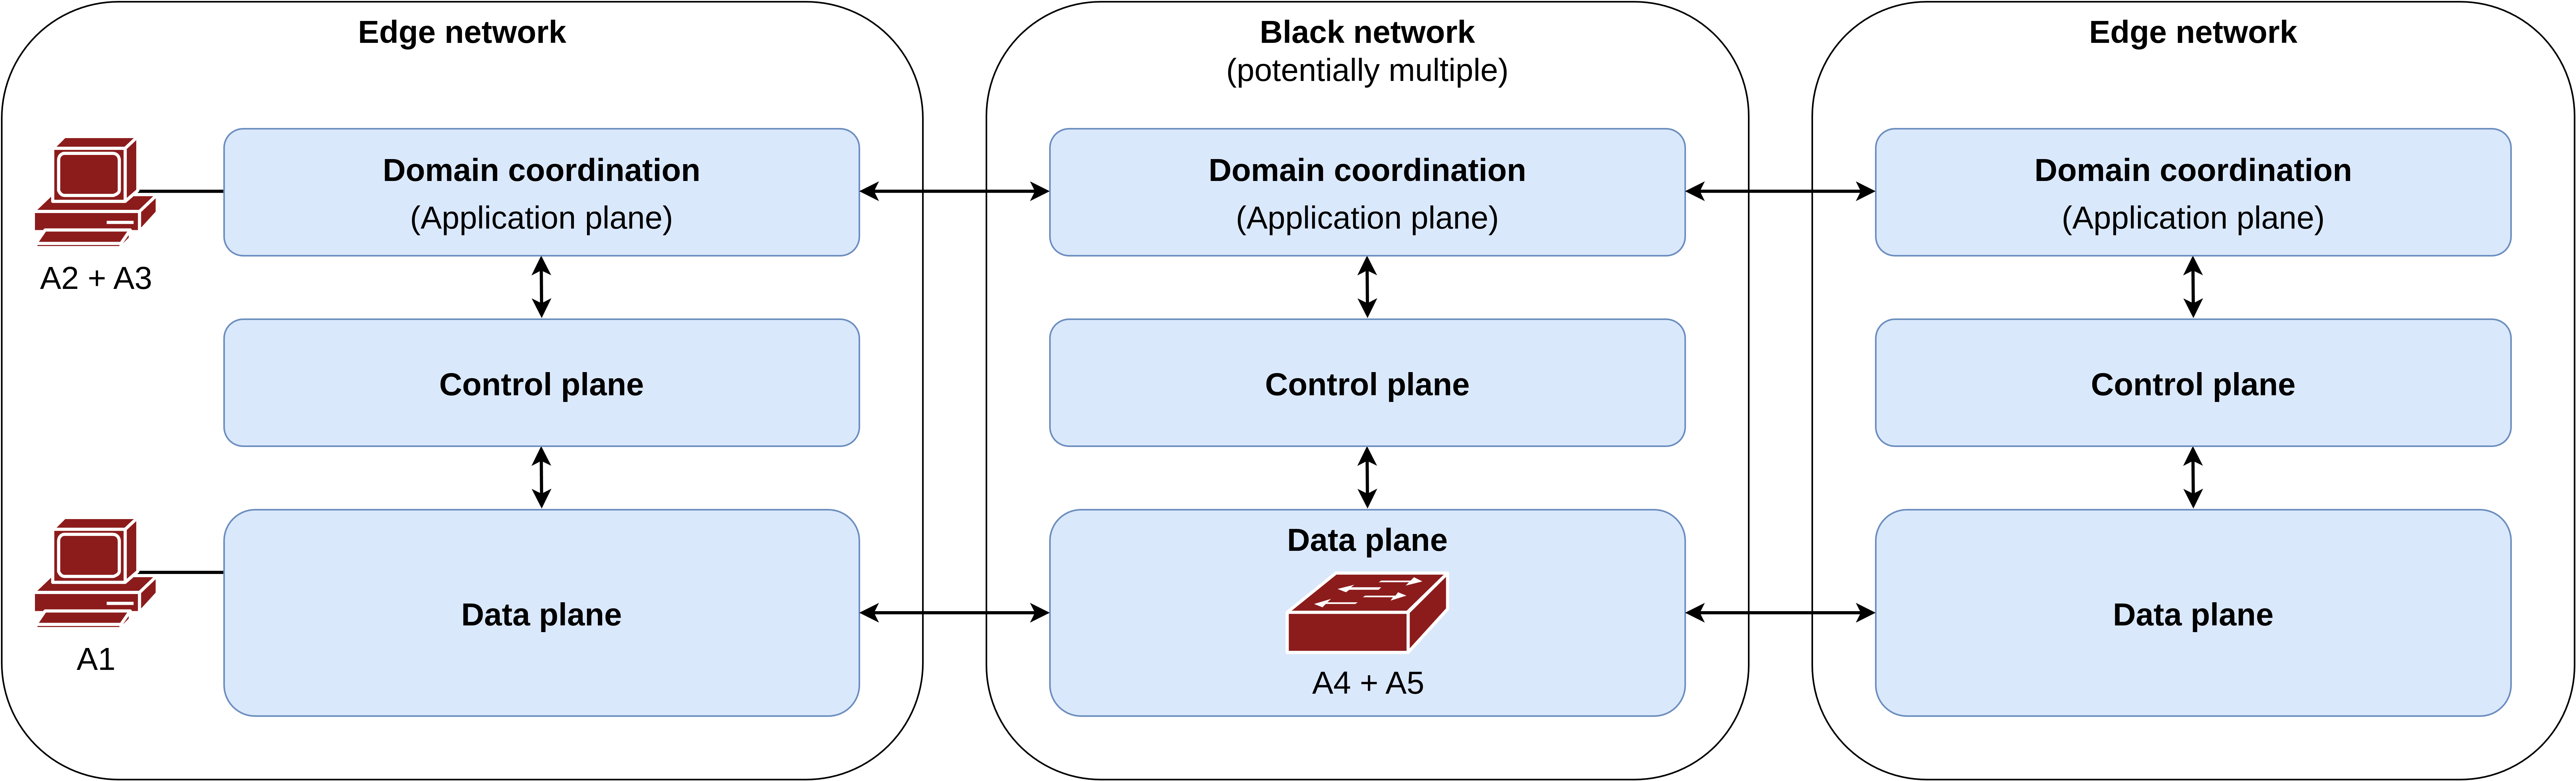
\includegraphics[width=\linewidth]{images/chapter_4/attacker_model.png}
  \caption[Attacker model]{Our attacker model indicating their location per domain and SDN plane.}
  \label{fig:attacker_model}
\end{figure}
\end{landscape}

\section{Scenarios}
\label{scenarios}
We will test three scenarios in total. The first scenario will provide a base case for our two other slicing-enabled scenarios, of which one will be local and the other distributed.

\begin{description}[style=multiline, labelwidth=0.7cm]
    \item[\namedlabel{S1}{S1}] \textbf{Reference scenario} The base solution will consist of two simulated hosts, two attackers and two switches. Each switch is connected to one of the hosts, one of the attackers and to the other switch. This scenario can be seen in figure \ref{fig:scenario_1}.
    \begin{figure}[ht]
        \centering
        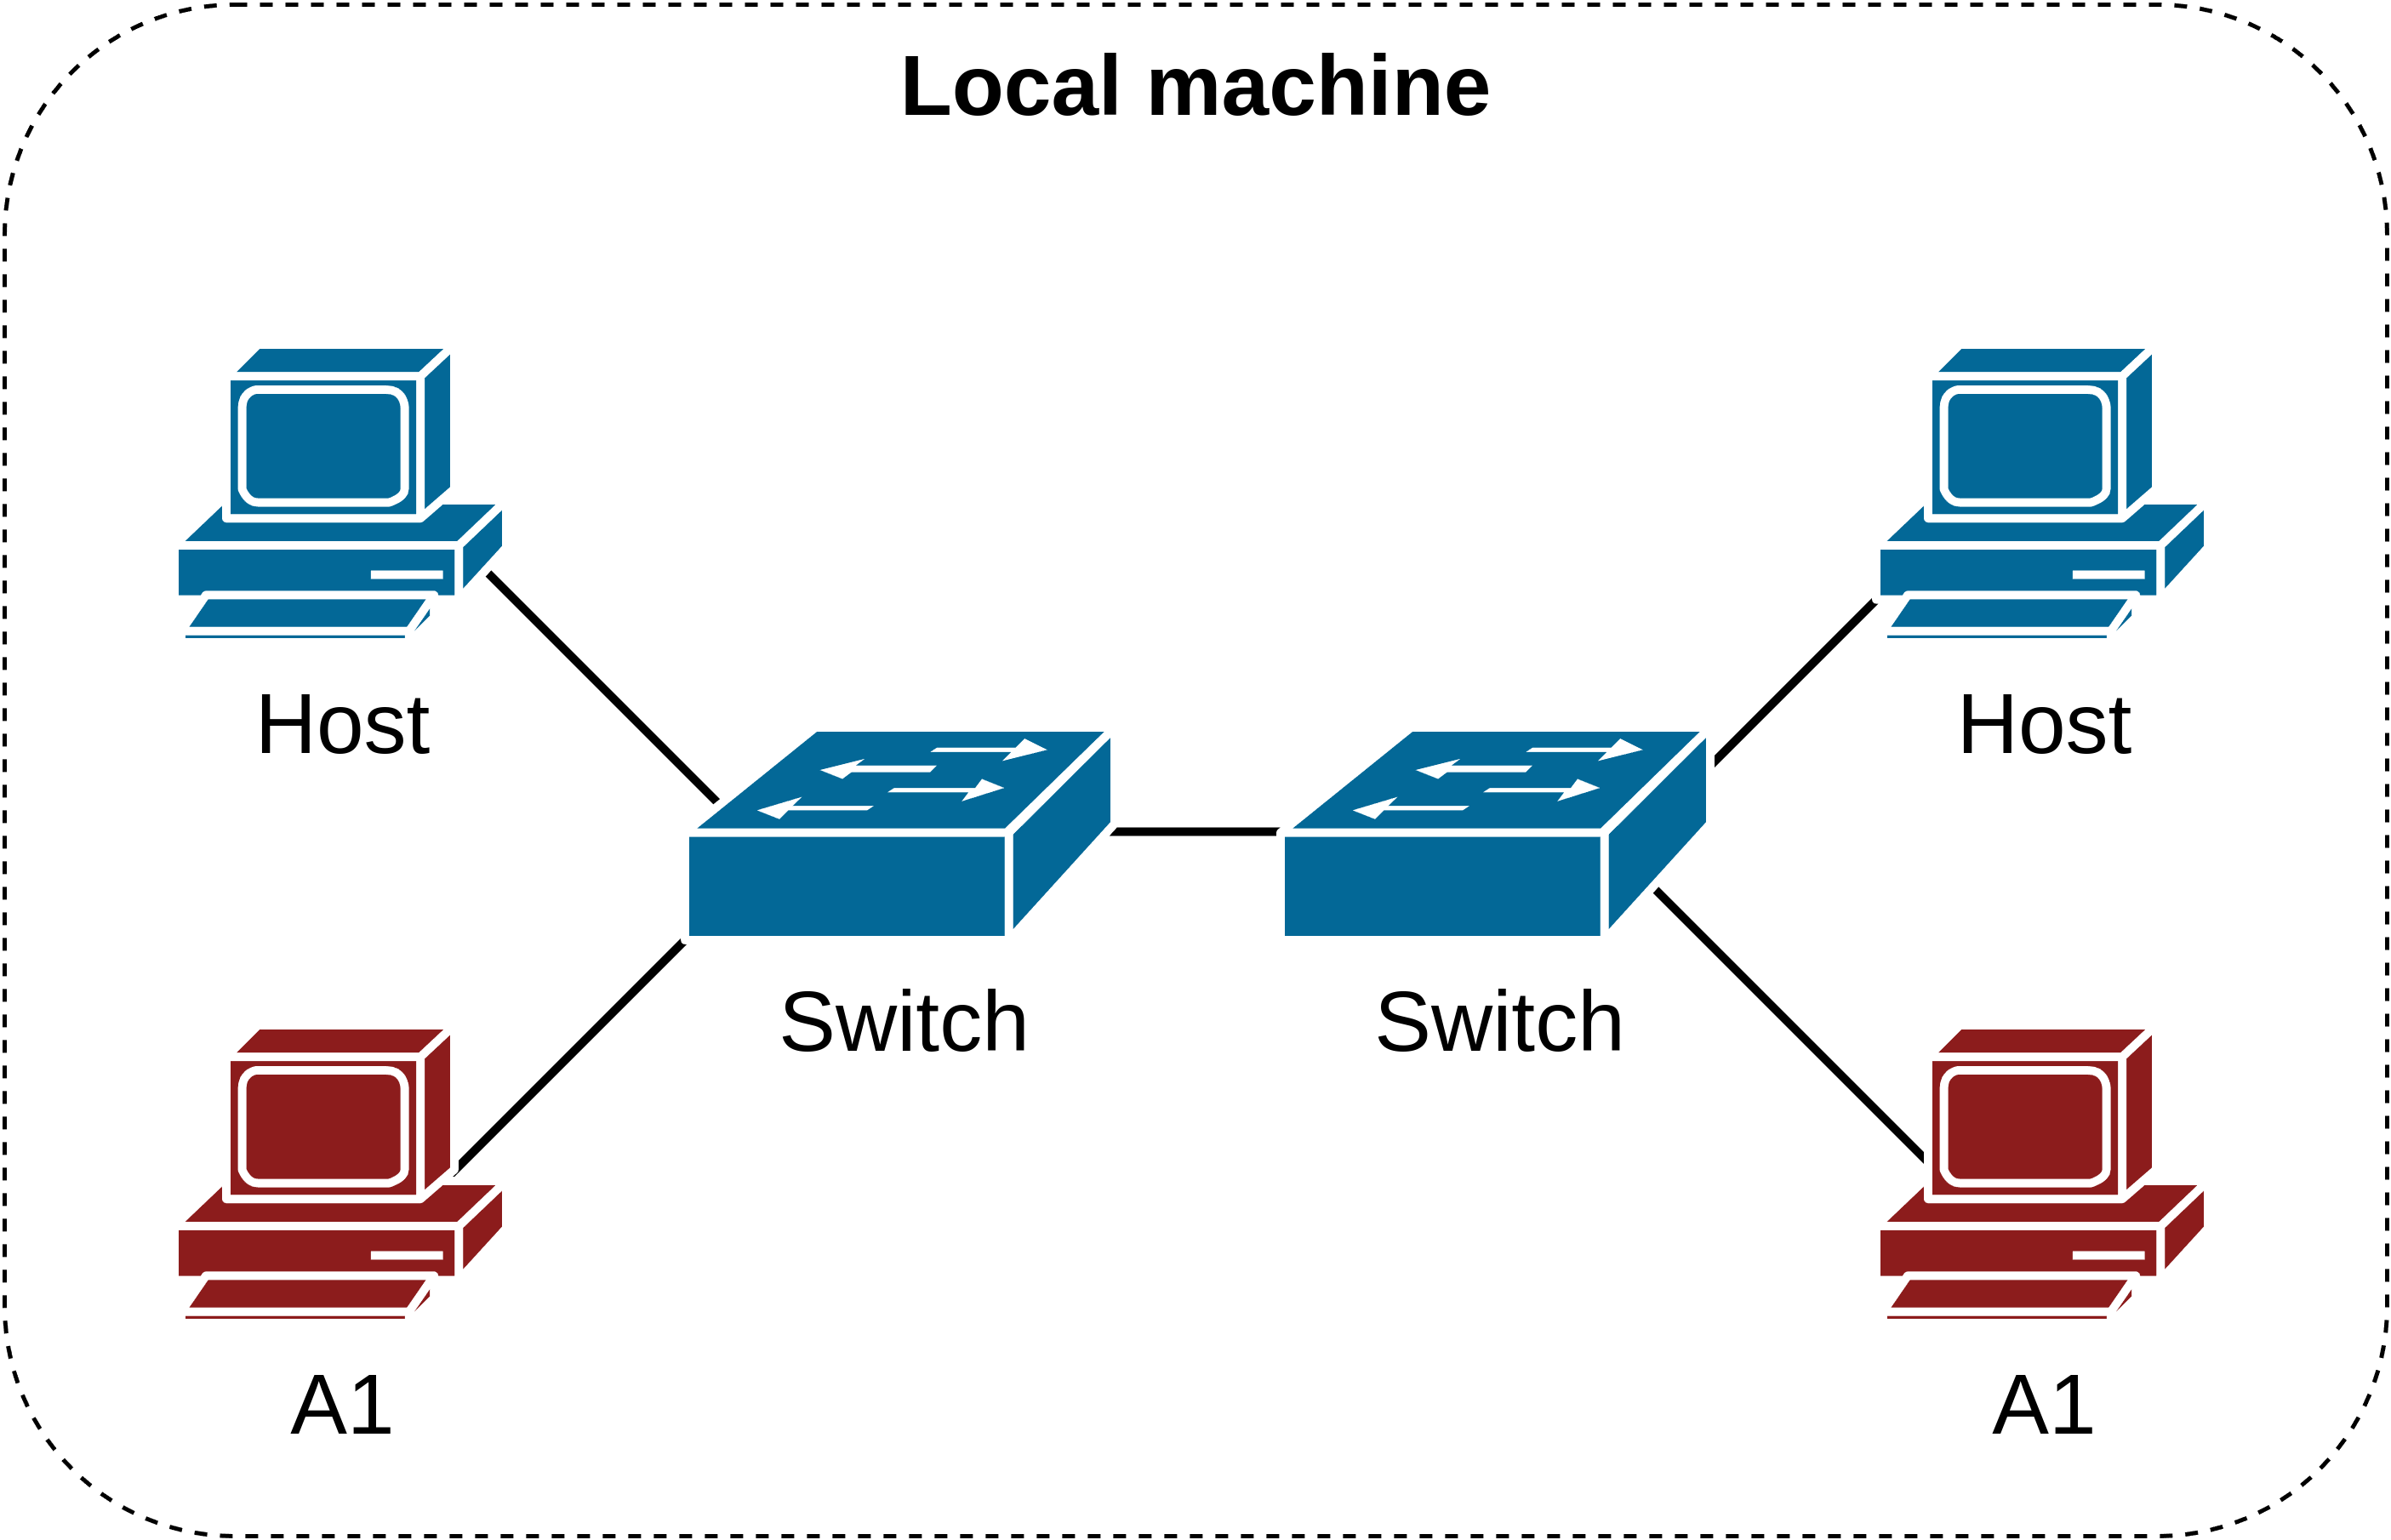
\includegraphics[width=12cm]{images/chapter_4/scenario_1.png}
        \caption[Validation Scenario 1]{Our first scenario \ref{S1} without network slicing.}
        \label{fig:scenario_1}
    \end{figure}
    \item[\namedlabel{S2}{S2}] \textbf{Local slicing scenario} For our first slicing scenario we will deploy our slicing solution emulating three domains with two edge networks and one black (semi-trusted) network between them. Each domain will have two slicing switches which the traffic of the slices has to pass. One of the simulated hosts will be created on each edge. This scenario can be seen in figure \ref{fig:scenario_2}.
    \begin{figure}[ht]
        \centering
        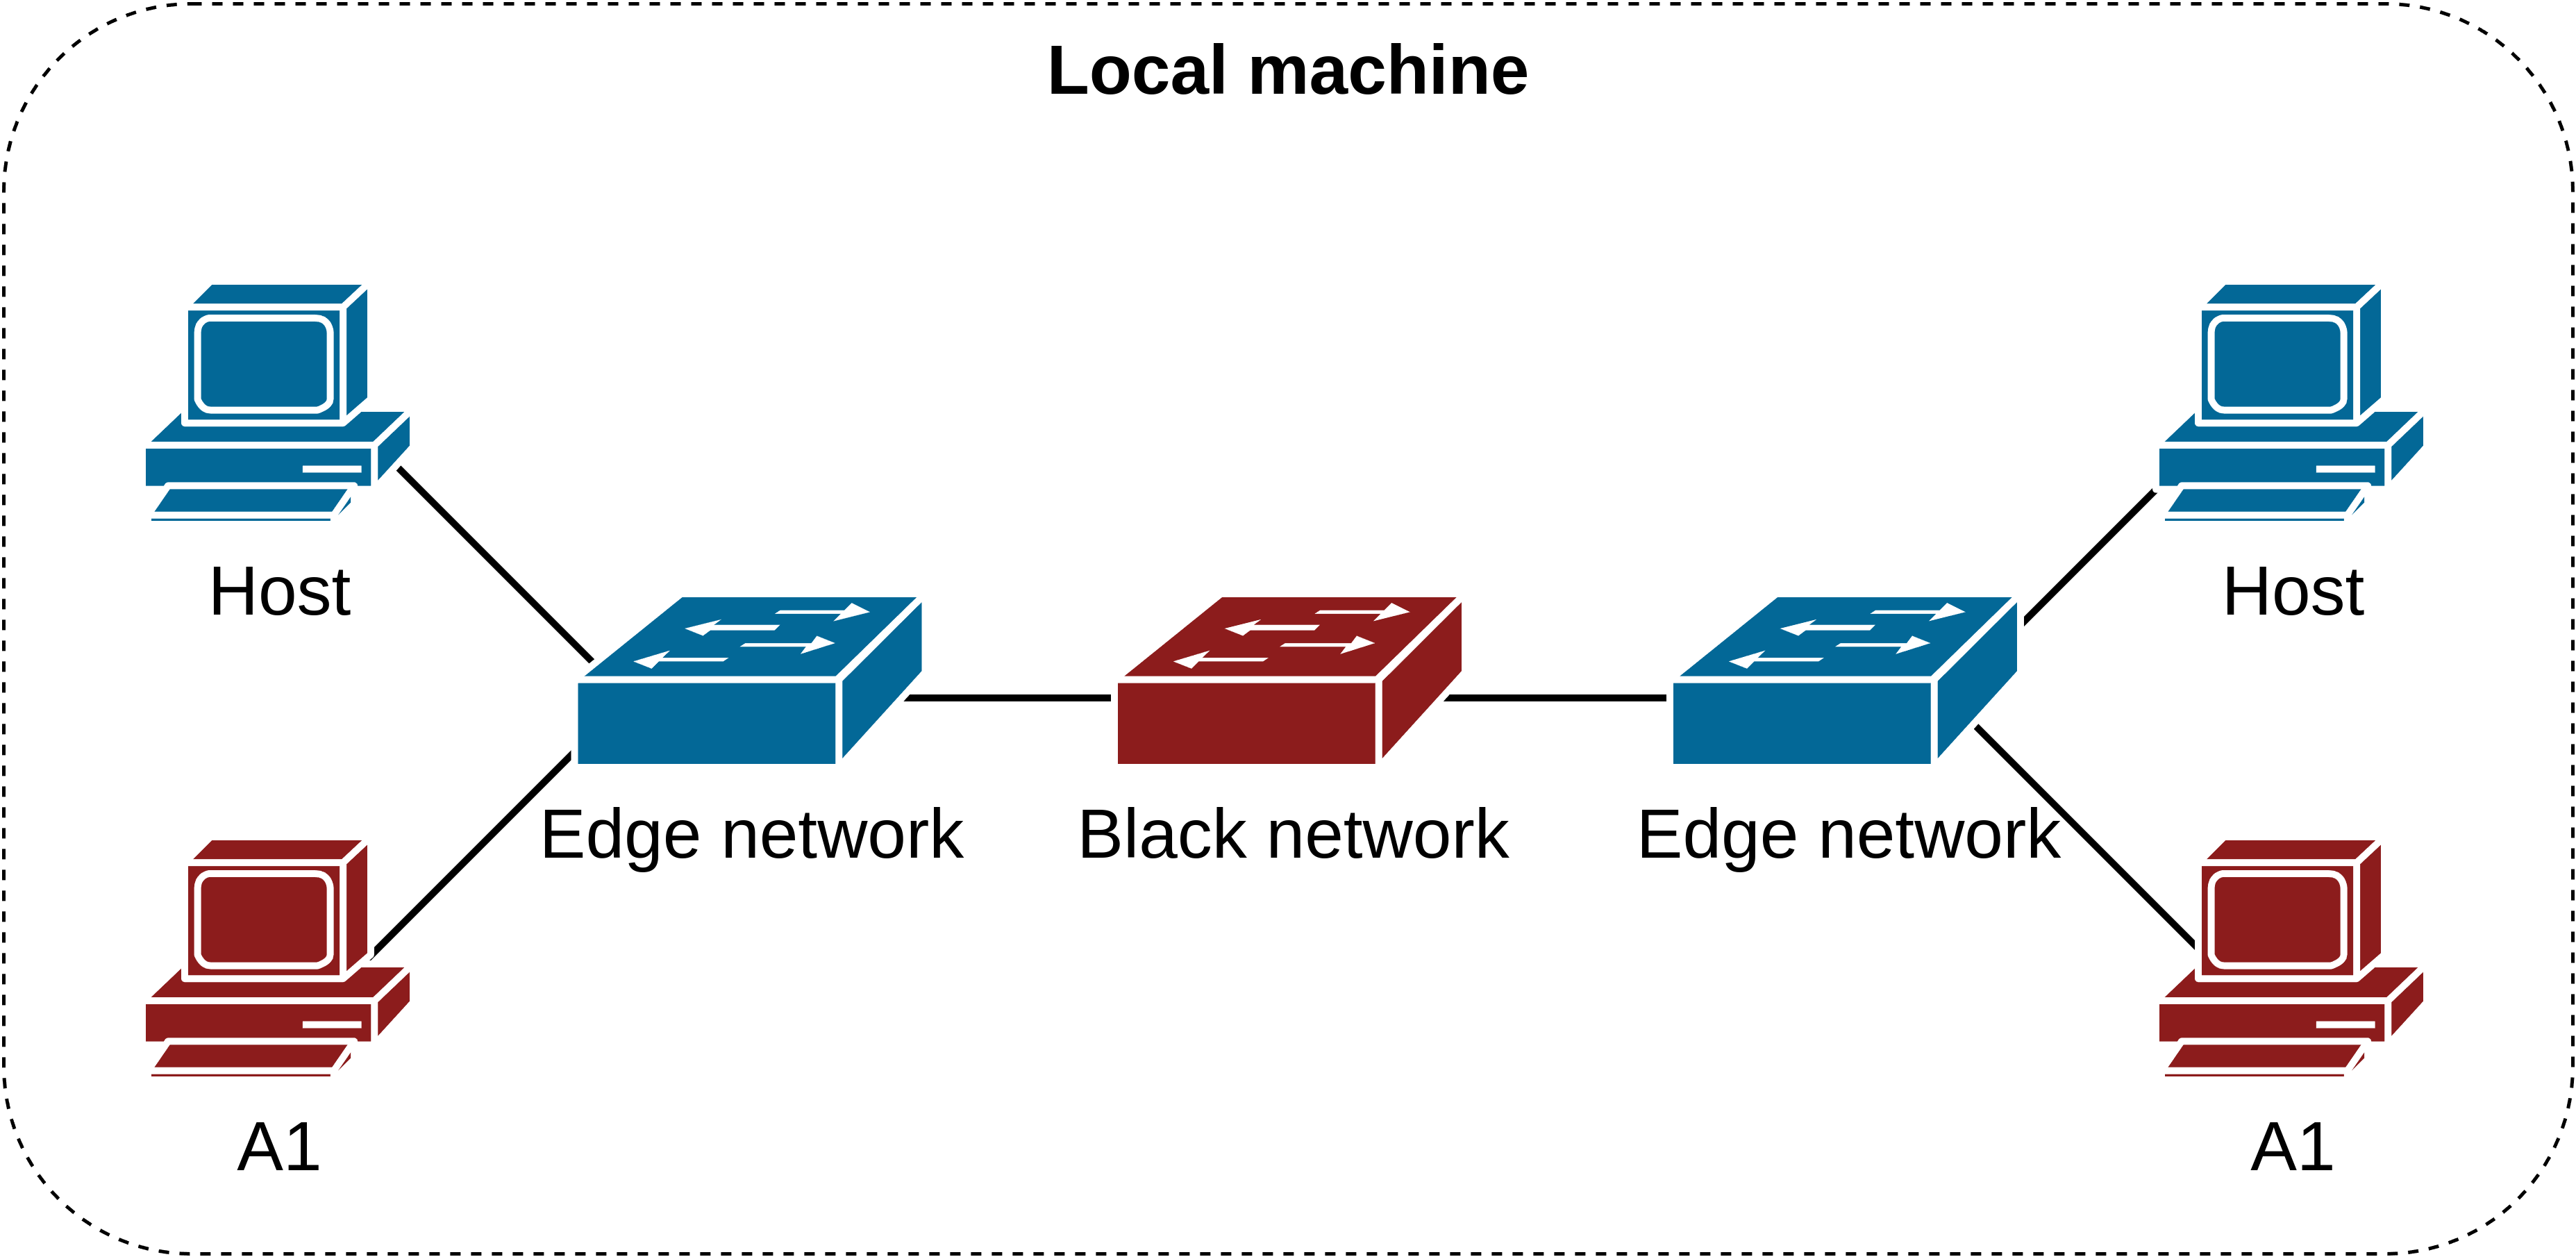
\includegraphics[width=\textwidth]{images/chapter_4/scenario_2.png}
        \caption[Validation Scenario 2]{Our second scenario \ref{S2} with network slicing across three domains running on a local test setup (one machine).}
        \label{fig:scenario_2}
    \end{figure}
    \item[\namedlabel{S3}{S3}] \textbf{Remote slicing scenario} As the last scenario we will deploy the previous scenario to three different servers that are connected via 10G links to an Aruba 2930F switch. Each server will contain one entire simulated domain. We hope that by this scenario we can observe some real-world performance characteristics when utilizing real links in our test environment. This scenario can be seen in figure \ref{fig:scenario_3}.
    \begin{figure}[ht]
        \centering
        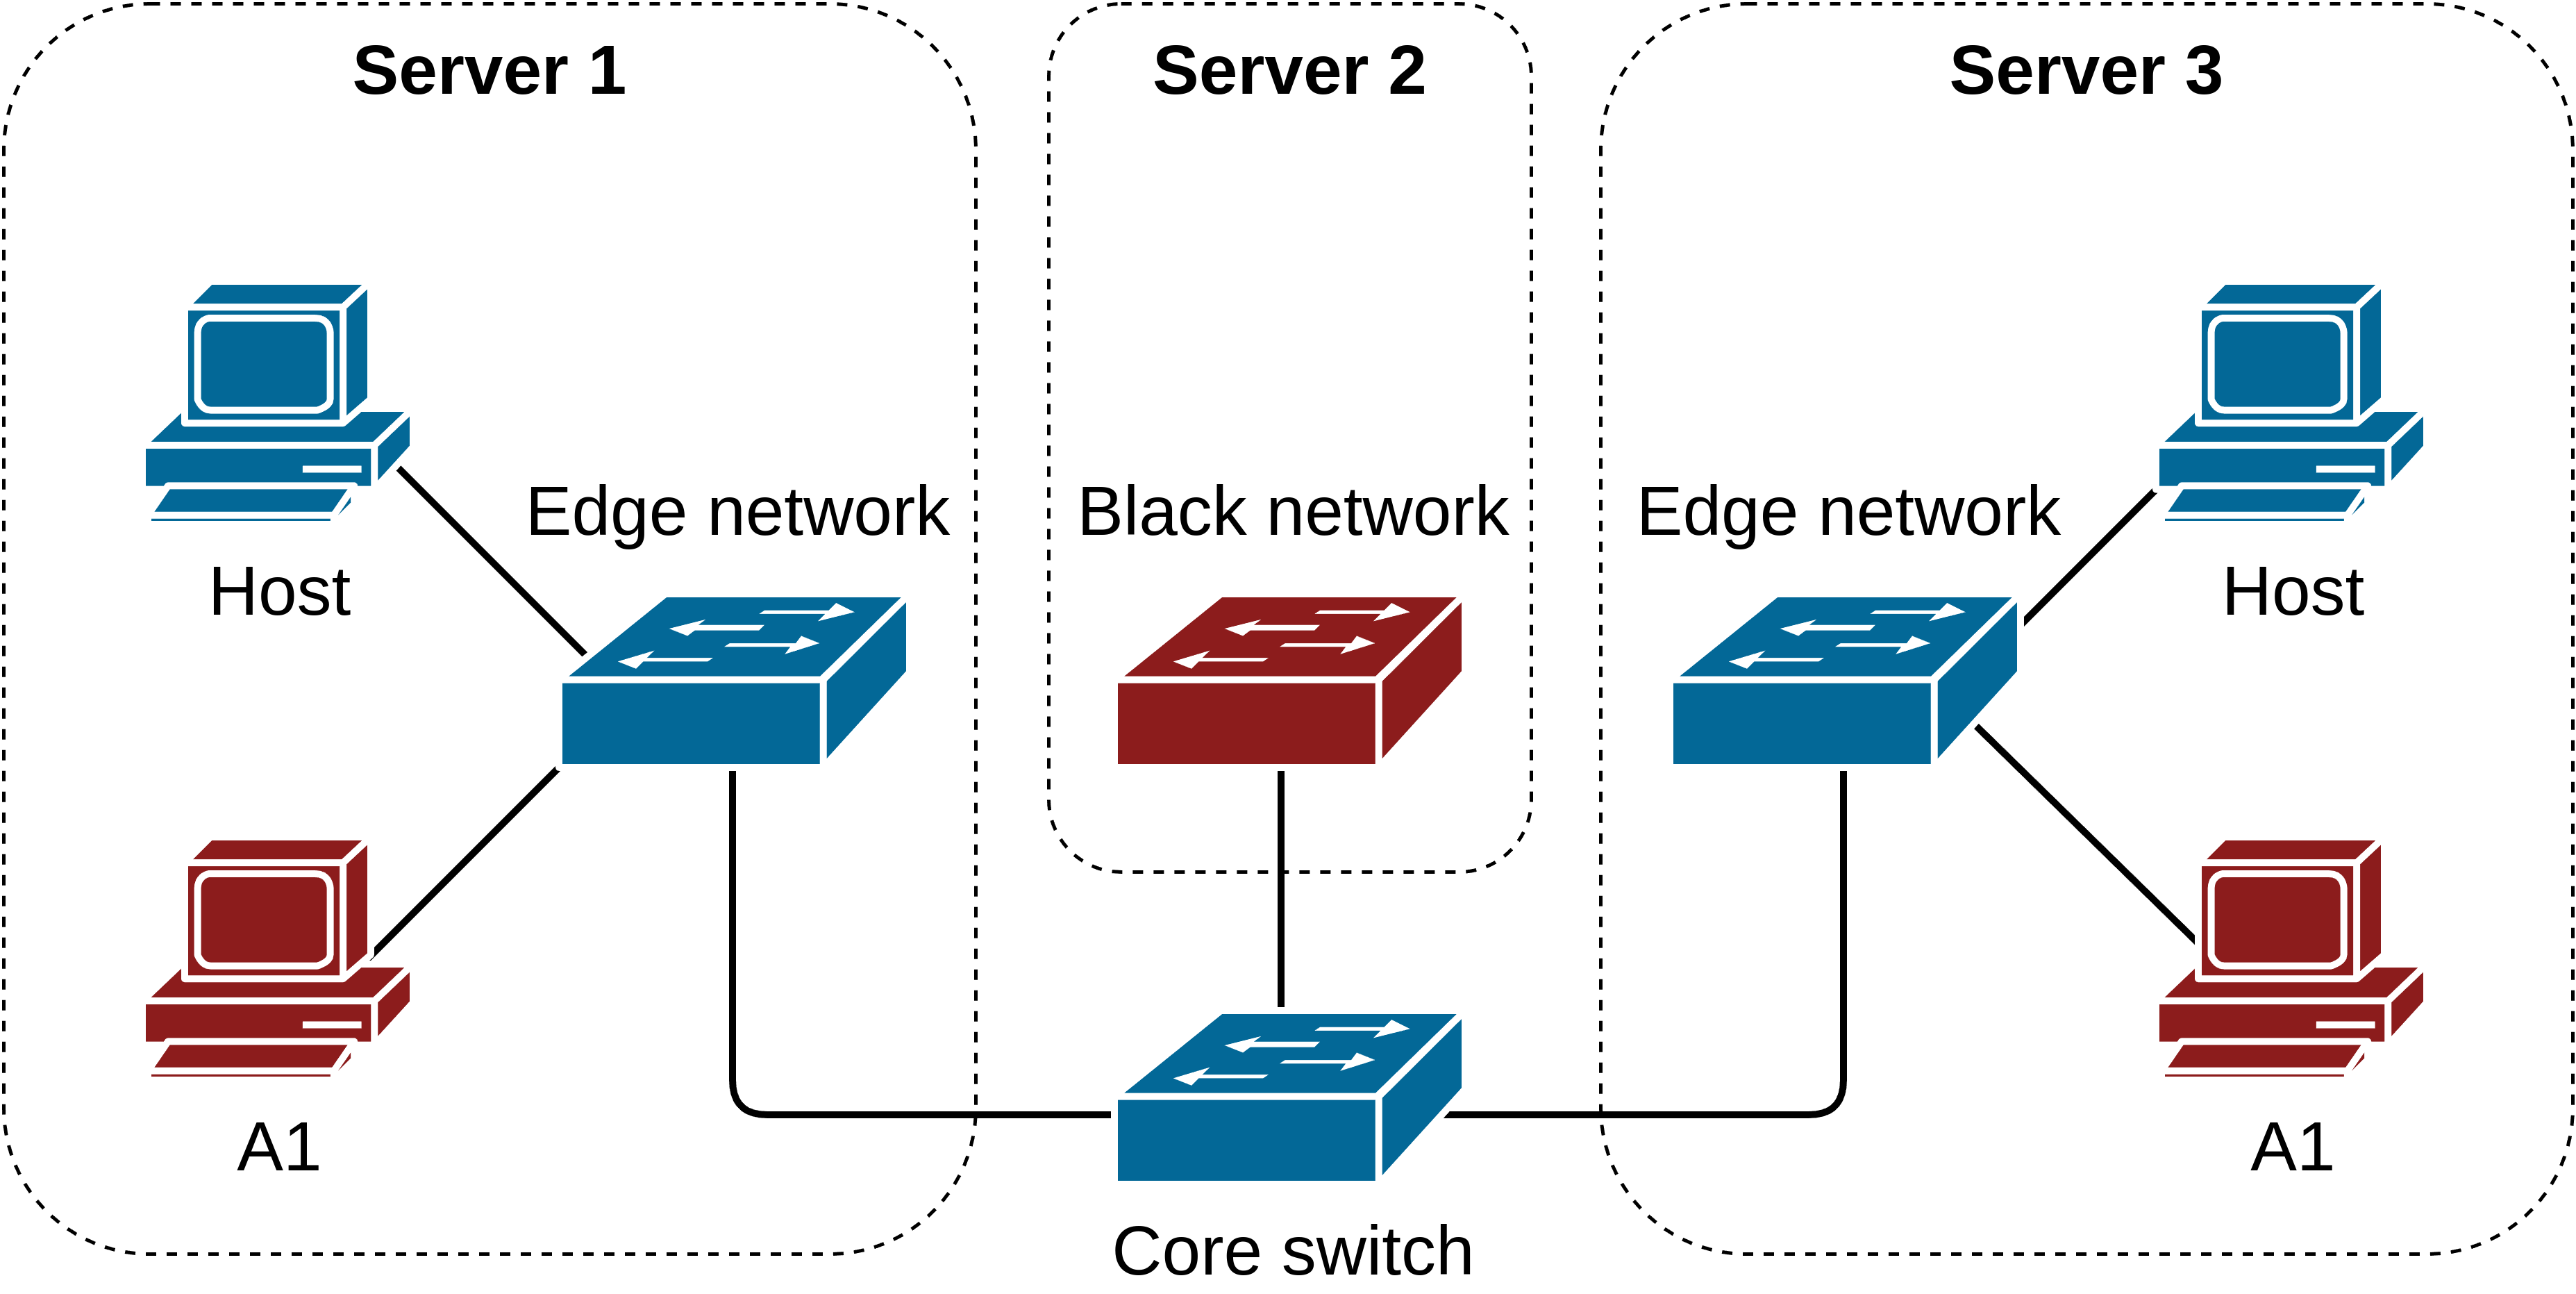
\includegraphics[width=\textwidth]{images/chapter_4/scenario_3.png}
        \caption[Validation Scenario 3]{Our last scenario \ref{S3} with network slicing across three domains, deploying one domain per server each. The three servers are connected via a switch.}
        \label{fig:scenario_3}
    \end{figure}
\end{description}

%The base solution will consist of two simulated hosts, two attackers and two switches. Each switch is connected to one of the hosts, one of the attackers and to the other switch. The attackers share the link between the switches with the normal host. The attacker \ref{A1} will then become active and attempt to disrupt the communication between the hosts. Furthermore we will employ attacker \ref{A4} to eavesdrop traffic between the switches. \ref{A2} and \ref{A3} do not apply since there is no slicing infrastructure.

%For our first slicing scenario we will deploy our slicing solution emulating 3 domains with two edge networks and one black (semi-trusted) network between them. We will place one attacker each in the edges to spam a slice between them as attacker \ref{A1}. We will deploy \ref{A4} on a link in the black network and deploy \ref{A2} and \ref{A3} to the application plane.

%As the last scenario we will deploy the previous scenario to three different servers that are connected via 10G links to an Aruba 2930F switch. Each server will contain one entire simulated domain. We hope that by this scenario we can observe some real-world performance characteristics when utilizing real links in our test environment.

For each scenario we will try to establish two network slices in total. As an example, we want to control a robot on the other side by receiving a video stream and maintaining a bidirectional control and feedback stream, as in our use case for the surgery.

One slice will thus be unidirectional and streaming media content. We will allocate 8Mbit/s to this slice, because this encompasses streaming of HD video (according to the FCC \cite{fcc}). We require a relatively small loss rate for this to not skip frames on the video stream, but loosing single packets and skipping a frame will not be too much of an issue. Jitter may occur as we can buffer our video stream data for short amounts of time, however we want our latency to be low so our frames appear in almost real time.

For the bidirectional control and feedback slice, we need far less bandwidth. The loss rate needs to be lower than with the video stream to be in control at all times. Also we require a low latency and low jitter to be able to react in real time and without any inaccurate movements. We will thus apply the resource guarantees in table \ref{table:slices} to all of our scenarios.

\begin{table}[ht]
    \centering
    \begin{tabular}{ |c|c|c| }
    \hline
    \textbf{Metric} & \textbf{Media} & \textbf{Control} \\
    \hline
         Bandwidth & $\geq$ 8Mbit/s & $\geq$ 100Kbit/s \\
         Latency   & $<$ 5ms     & $<$ 3ms      \\
         Jitter    & $<$ 0.5ms  & $<$ 0.3ms   \\
         Loss rate & $<$ 0.01\% & $<$ 0.001\% \\
    \hline
    \end{tabular}
    \caption[Slice QoS guarantees in our remote surgery example]{The guarantees we wish to meet with our slices concerning our remote surgery example.}
    \label{table:slices}
\end{table}

The robot example including the bandwidth requirements is taken from Fuhrberg et al. \cite{SE4} in order to be able to compare their solution against our redesigned solution. The values for latency, jitter and loss rate have been altered to reflect our goals and generally provide more strict requirements.

\section{Measurements}
\label{measurements}
Measurements on the resources of a slice will be performed by sending continuous traffic according to the slice specifications through the slice. By sending the traffic and observing the packets reaching the other and, we can obtain measurements on whether the slices upheld their guarantees in this specific situation or not.

To send the traffic and observe their result, we will use three different tools:

\paragraph{Iperf3} \cite{iperf3} is a network bandwidth testing tool that also provides data on packet drops and connection jitter. It supports both UDP and TCP.

\paragraph{Iputils-ping} \cite{iputils} is a network latency testing tool that provides data on latency, packet drops and jitter. We will not generate traffic using ping, but will rather use it for latency measurements while \textit{iperf3} sends continuous traffic. It will use ICMP as protocol.

\paragraph{Sockperf} \cite{sockperf} is a network bandwidth and latency testing tool that provides data on bandwidth, packet drops, latency and jitter. It supports both UDP and TCP.

\paragraph{} More details on this can be seen in table \ref{table:measurements}. We will thus be able to obtain each metric from at least two tools, providing us with the ability to verify their result.

\begin{table}[ht]
    \centering
    \begin{tabular}{ |c|c|c|c|c| }
    \hline
    \textbf{Tool} & \textbf{Bandwidth} & \textbf{Packet drops} & \textbf{Latency} & \textbf{Jitter}  \\
    \hline
         IPerf3   & \ding{51} & UDP only  & TCP only  & UDP only  \\
         Ping     & \ding{55} & \ding{51} & \ding{51} & \ding{51} \\
         Sockperf & \ding{51} & \ding{51} & \ding{51} & \ding{51} \\
    \hline
    \end{tabular}
    \caption[Measurements of different tools]{The measurements obtained on our different tools}
    \label{table:measurements}
\end{table}

%For each scenario and each attacker (apart from \ref{A4}), we will investigate the availability of our slice and measure our available bandwidth, loss rate, latency and jitter while sending the amount of traffic we reserved. We will compare our results to the values that we requested in the individual slice.

%For the eavesdropping attacker \ref{A4} we will listen on the link between the switches for the non-edgeslicing scenario and on a link in the black network for the edge-slicing scenarios.

\section{Experiments}
\label{methodology_experiments}
\iffalse
For each experiment
\begin{itemize}
    \item Give the experiment a number (e.g. E1)
    \item What do we want to test
    \item How (including attackers)
    \item With what (algorithms for test and attacker algorithm)
    \item Expectations
    \item How should be evaluated
\end{itemize}
$\Rightarrow$ Outcome and expectation validation in validation chapter later
\fi

In this section we are now going to state the experiments that we are going to perform. We will perform one experiment for each attacker, apart from the integrity attacker (see below for more info on this). The experiments are numbered the same as the attackers.

\begin{description}[style=multiline, labelwidth=0.7cm]
    \item[\namedlabel{E1}{E1}] \textbf{Slice availability and resilience} In this experiment we want to test whether the slice isolation is working as expected. For this, we will place one attacking host on each of the edges, which send traffic along the same path that our slice is taking by using \textit{hping3} \cite{hping3}. Hping3 is a tool to spam traffic on network interfaces.

    We will establish our test slices specified in section \ref{scenarios} and obtain base measurements using the three tools mentioned in section \ref{measurements} without activating the attackers yet. For scenario \ref{S1} where no slicing setup is available, we will perform all measurements without setting up slices in advance. Afterwards we will activate the attackers and increase the traffic produced by hping3 while continuing our measurements until either the isolation fails or the attackers have reached their maximum possible capacity. The maximum possible computational power the attackers get in a simulated environment is 30 out of 32 in our local environments \ref{S1} and \ref{S2}, and 3 out of 4 per server in our remote slicing environment \ref{S3}, so there is still some computational capacity available for the scenarios, which is more than generous to the attackers.

    We will also install a large number of flow entries with higher priority on the switches subsequently to test whether a large number of flows (number of attacker threads mentioned above) compromises our isolation efforts. The maximum number of flows uses the same reasoning as above. In a real-world network we can also decide how many local participants may route their traffic via our switches, where we need to scale our infrastructure according to the number of participants. It thus makes sense to determine attacker capacity by our own capacity, apart from the fact that we are locked to it anyways by sheer capacity we possess in our simulated environments.

    If the isolation fails, then we have not reached our isolation requirement \ref{R1}. If on the other hand the attackers reach their capacity limit, spam flows have been installed and there is still no violation of isolation, the experiment has succeeded, due to the isolation being better than the traffic generation capacity of the system. This would validate our protection goals of availability (\ref{P3}) and resilience (\ref{P4}).

    We would expect that our slice is isolated from this other traffic and no effects can be seen on the slice concerning the additional traffic in the system.

    \item[\namedlabel{E2}{E2}] \textbf{Application plane availability and resilience (1)} In this experiment we will try to perform DoS on the application plane by spamming unauthenticated requests on the domain coordinator. We will spam the domain coordinator by using a python script that has been self developed and can be found in the sources. It uses multiple threads to spam http requests.

    For reproducing purposes, we will measure our achieved request rate by examining the output from our script.

    We expect the coordinator to go down, because we have not protected it against http spam yet. We will validate this by starting the spam on the coordinator and then performing a slice request a couple of seconds later. We expect our request to not be replied to.

    \item[\namedlabel{E3}{E3}] \textbf{Application plane availability and resilience (2)} In this experiment we will use the same approach as in experiment \ref{E2}, but will rather spam authenticated requests. We will send the requests at a lower rate, because we want the coordinator to have to work on them. For authentication we will use a separate authentication token that is assigned to the attacker first and afterwards we will use the token from our slice requesting host to determine what happens when a token is stolen from a host.

    We expect the coordinator to stay up, because there is a rate limit and an allocation limit for slice requests from one identity in place. The spam will thus also not propagate through the network. We will validate this by starting the spam on the coordinator and then performing a slice request a couple of seconds later.

    In the case of using the adversary token to spam slice requests we expect our request of a slice to go through. In the case that our host token is being used to spam slice requests, we expect to be denied our slice allocation because we already have too many open slices under our identity.

    \item[\namedlabel{E4}{E4}] \textbf{Slice confidentiality} In this experiment we try to break confidentiality by eavesdropping on the switches of the black network (protection goal \ref{P1}). To achieve this, we are going to use a tool called \textit{tcpdump} \cite{tcpdump} to dump packets passing a black network switch. Tcpdump is a traffic sniffer that will collect packets passing on an interface either to console or to a file.

    For this, we will establish slices (apart from scenario \ref{S1} where no slicing is available) according to our scenario section (\ref{scenarios}). We will then send secret traffic along the slice using a simple python while loop (the implementation can be seen below) on the slice initiator that is sending UDP traffic to the remote host. We will then start sniffing on an appropriate switch port of the black network.

\begin{lstlisting}[language=python]
import socket

# Create a UDP socket
socket = socket.socket(socket.AF_INET, socket.SOCK_DGRAM)

while True:
    # Send a packet with secret content to the remote host
    sock.sendto(b"This traffic should be encrypted!",
                ("<dest_ip>", <dest_port>))
\end{lstlisting}

    We expect to see only encrypted traffic on the black network that moves from one tunnel endpoint to the other and vice versa. This experiment succeeds when the traffic is encrypted, or fails when it is not.

    %\item[\namedlabel{E5}{E5}] \textbf{Slice integrity} In this final experiment we will try to replay packets from a black network switch by capturing it and delivering it twice. We will use a \textit{qdisc} (part of \textit{iproute2} \cite{iproute2}) for this to multiply our traffic and send every ingress packet twice.

    %To test this, we will establish our slices (apart from scenario \ref{S1} again where no slicing is available) and then install our traffic duplication qdisc on a black network switch. Afterwards we will start sending continuous traffic from one host using our python UDP loop as in experiment \ref{E4}. We will then execute \textit{tcpdump} \cite{tcpdump} on the other host and look for packets that have been delivered twice with the same content.

    %We expect to see no duplicates being delivered on our receiving host. If there are no duplicates, the experiment succeeds. If there are, we have broken integrity and the experiment fails.

    %While this experiment does not cover all possible integrity violations, the integrity on the black network can be assumed to be protected because our utilization of the wireguard protocol. The wireguard whitepaper proves the resilience of wireguard to replay attacks by using nonces and to message forgery by using authentication tags \cite{wireguard}.

    %This experiment has been removed and integrated into experiment E4. We rather claim integrity as by design of wireguard, because the experiment E5 does not cover all attacker angles.

\end{description}

We do not conduct a fifth experiment for the fifth attacker, because we already check with experiment \ref{E4} that our traffic is passing the black network through our wireguard tunnel. Apart from provably encrypting traffic, wireguard tunnels also protect data integrity according to their whitepaper \cite{wireguard}. As there is formal proof for this we can be sure that conducting an arbitrary attack on integrity will not lead to a violation of integrity. Experiment \ref{E4} thus also covers integrity, which is our protection goal \ref{P2}.

\newcolumntype{P}{>{\centering\arraybackslash}p{.19\textwidth}}
\begin{table}[ht]
    \centering
    \begin{tabular}{|c|P|P|P|P|}
         \hline
         \textbf{Exp} & \textbf{\ref{P1}} & \textbf{\ref{P2}} & \textbf{\ref{P3}} & \textbf{\ref{P4}} \\
         ~ & Confidentiality & Integrity & Availability & Resilience \\
         \hline
         \ref{E1} & ~ & ~ & \ding{51}$^D$ & \ding{51}$^D$ \\
         \ref{E2} & ~ & ~ & \ding{51}$^A$ & \ding{51}$^A$ \\
         \ref{E3} & ~ & ~ & \ding{51}$^A$ & \ding{51}$^A$ \\
         \ref{E4} & \ding{51}$^D$ & \ding{51}$^D$ & ~ & ~ \\
         \hline
    \end{tabular}
    \caption[Protection goal coverage by experiments]{Protection goal coverage by experiments. A: Targets application plane. D: Targets data plane (slice).}
    \label{table:experiment_coverage}
\end{table}

In table \ref{table:experiment_coverage} we give an overview over our experiment coverage.